\batchmode
\makeatletter
\def\input@path{{/Users/Adam/Dropbox/Stat215A-2013/Labs/Lab2/Lab//}}
\makeatother
\documentclass[english]{article}\usepackage{graphicx, color}
%% maxwidth is the original width if it is less than linewidth
%% otherwise use linewidth (to make sure the graphics do not exceed the margin)
\makeatletter
\def\maxwidth{ %
  \ifdim\Gin@nat@width>\linewidth
    \linewidth
  \else
    \Gin@nat@width
  \fi
}
\makeatother

\IfFileExists{upquote.sty}{\usepackage{upquote}}{}
\definecolor{fgcolor}{rgb}{0.2, 0.2, 0.2}
\newcommand{\hlnumber}[1]{\textcolor[rgb]{0,0,0}{#1}}%
\newcommand{\hlfunctioncall}[1]{\textcolor[rgb]{0.501960784313725,0,0.329411764705882}{\textbf{#1}}}%
\newcommand{\hlstring}[1]{\textcolor[rgb]{0.6,0.6,1}{#1}}%
\newcommand{\hlkeyword}[1]{\textcolor[rgb]{0,0,0}{\textbf{#1}}}%
\newcommand{\hlargument}[1]{\textcolor[rgb]{0.690196078431373,0.250980392156863,0.0196078431372549}{#1}}%
\newcommand{\hlcomment}[1]{\textcolor[rgb]{0.180392156862745,0.6,0.341176470588235}{#1}}%
\newcommand{\hlroxygencomment}[1]{\textcolor[rgb]{0.43921568627451,0.47843137254902,0.701960784313725}{#1}}%
\newcommand{\hlformalargs}[1]{\textcolor[rgb]{0.690196078431373,0.250980392156863,0.0196078431372549}{#1}}%
\newcommand{\hleqformalargs}[1]{\textcolor[rgb]{0.690196078431373,0.250980392156863,0.0196078431372549}{#1}}%
\newcommand{\hlassignement}[1]{\textcolor[rgb]{0,0,0}{\textbf{#1}}}%
\newcommand{\hlpackage}[1]{\textcolor[rgb]{0.588235294117647,0.709803921568627,0.145098039215686}{#1}}%
\newcommand{\hlslot}[1]{\textit{#1}}%
\newcommand{\hlsymbol}[1]{\textcolor[rgb]{0,0,0}{#1}}%
\newcommand{\hlprompt}[1]{\textcolor[rgb]{0.2,0.2,0.2}{#1}}%

\usepackage{framed}
\makeatletter
\newenvironment{kframe}{%
 \def\at@end@of@kframe{}%
 \ifinner\ifhmode%
  \def\at@end@of@kframe{\end{minipage}}%
  \begin{minipage}{\columnwidth}%
 \fi\fi%
 \def\FrameCommand##1{\hskip\@totalleftmargin \hskip-\fboxsep
 \colorbox{shadecolor}{##1}\hskip-\fboxsep
     % There is no \\@totalrightmargin, so:
     \hskip-\linewidth \hskip-\@totalleftmargin \hskip\columnwidth}%
 \MakeFramed {\advance\hsize-\width
   \@totalleftmargin\z@ \linewidth\hsize
   \@setminipage}}%
 {\par\unskip\endMakeFramed%
 \at@end@of@kframe}
\makeatother

\definecolor{shadecolor}{rgb}{.97, .97, .97}
\definecolor{messagecolor}{rgb}{0, 0, 0}
\definecolor{warningcolor}{rgb}{1, 0, 1}
\definecolor{errorcolor}{rgb}{1, 0, 0}
\newenvironment{knitrout}{}{} % an empty environment to be redefined in TeX

\usepackage{alltt}
\usepackage[T1]{fontenc}
\usepackage[latin9]{inputenc}
\usepackage{geometry}
\geometry{verbose,tmargin=1in,bmargin=1in,lmargin=1in,rmargin=1in}
\usepackage{fancyhdr}
\pagestyle{fancy}
\setlength{\parskip}{\smallskipamount}
\setlength{\parindent}{0pt}
\usepackage{amsthm}
\usepackage{amsmath}
% \usepackage{graphicx}
% \usepacakge{subfig}

\makeatletter

%%%%%%%%%%%%%%%%%%%%%%%%%%%%%% LyX specific LaTeX commands.
\providecommand{\LyX}{L\kern-.1667em\lower.25em\hbox{Y}\kern-.125emX\@}

%%%%%%%%%%%%%%%%%%%%%%%%%%%%%% Textclass specific LaTeX commands.
\numberwithin{equation}{section}
\numberwithin{figure}{section}

\@ifundefined{date}{}{\date{}}
%%%%%%%%%%%%%%%%%%%%%%%%%%%%%% User specified LaTeX commands.
\pagestyle{empty} 

\makeatother

\usepackage{babel}
\begin{document}

\title{Lab 4 - Cloud Data\\
Stat 215A, Fall 2014}


\author{Ruoxi Jia}

\maketitle
\section{Introduction}
In this Lab, our mission is to predict cloud in the polar regions using a group of selected features. Firstly, we carry out EDA to explore feature distribution and their potential correlations. Then based on EDA observation, three features are selected as discriminators of cloud detection. Secondly, variety of  statistical and non-probabilistic models are fitted to the data and compared with each other with both visual and quantitative methods. Finally, we try to diagnose fitted models and explore error patterns for possible model improvement.

\section{EDA}
The dataset for cloud identification is not so multidimensional as to require use of tremendous dimensionality reduction. Rather, we can identify, within each feature, characteristics that permit greater precision and generality of our results.

\subsection{Probability mass by category}
The most direct exploration of the data involves an exploration of the 1-D 
features and the distribution of categories within. The most useful density 
plots in our data set are demonstrated in Fig.??. 


\begin{figure}[!h]
\begin{tabular}{cc}
  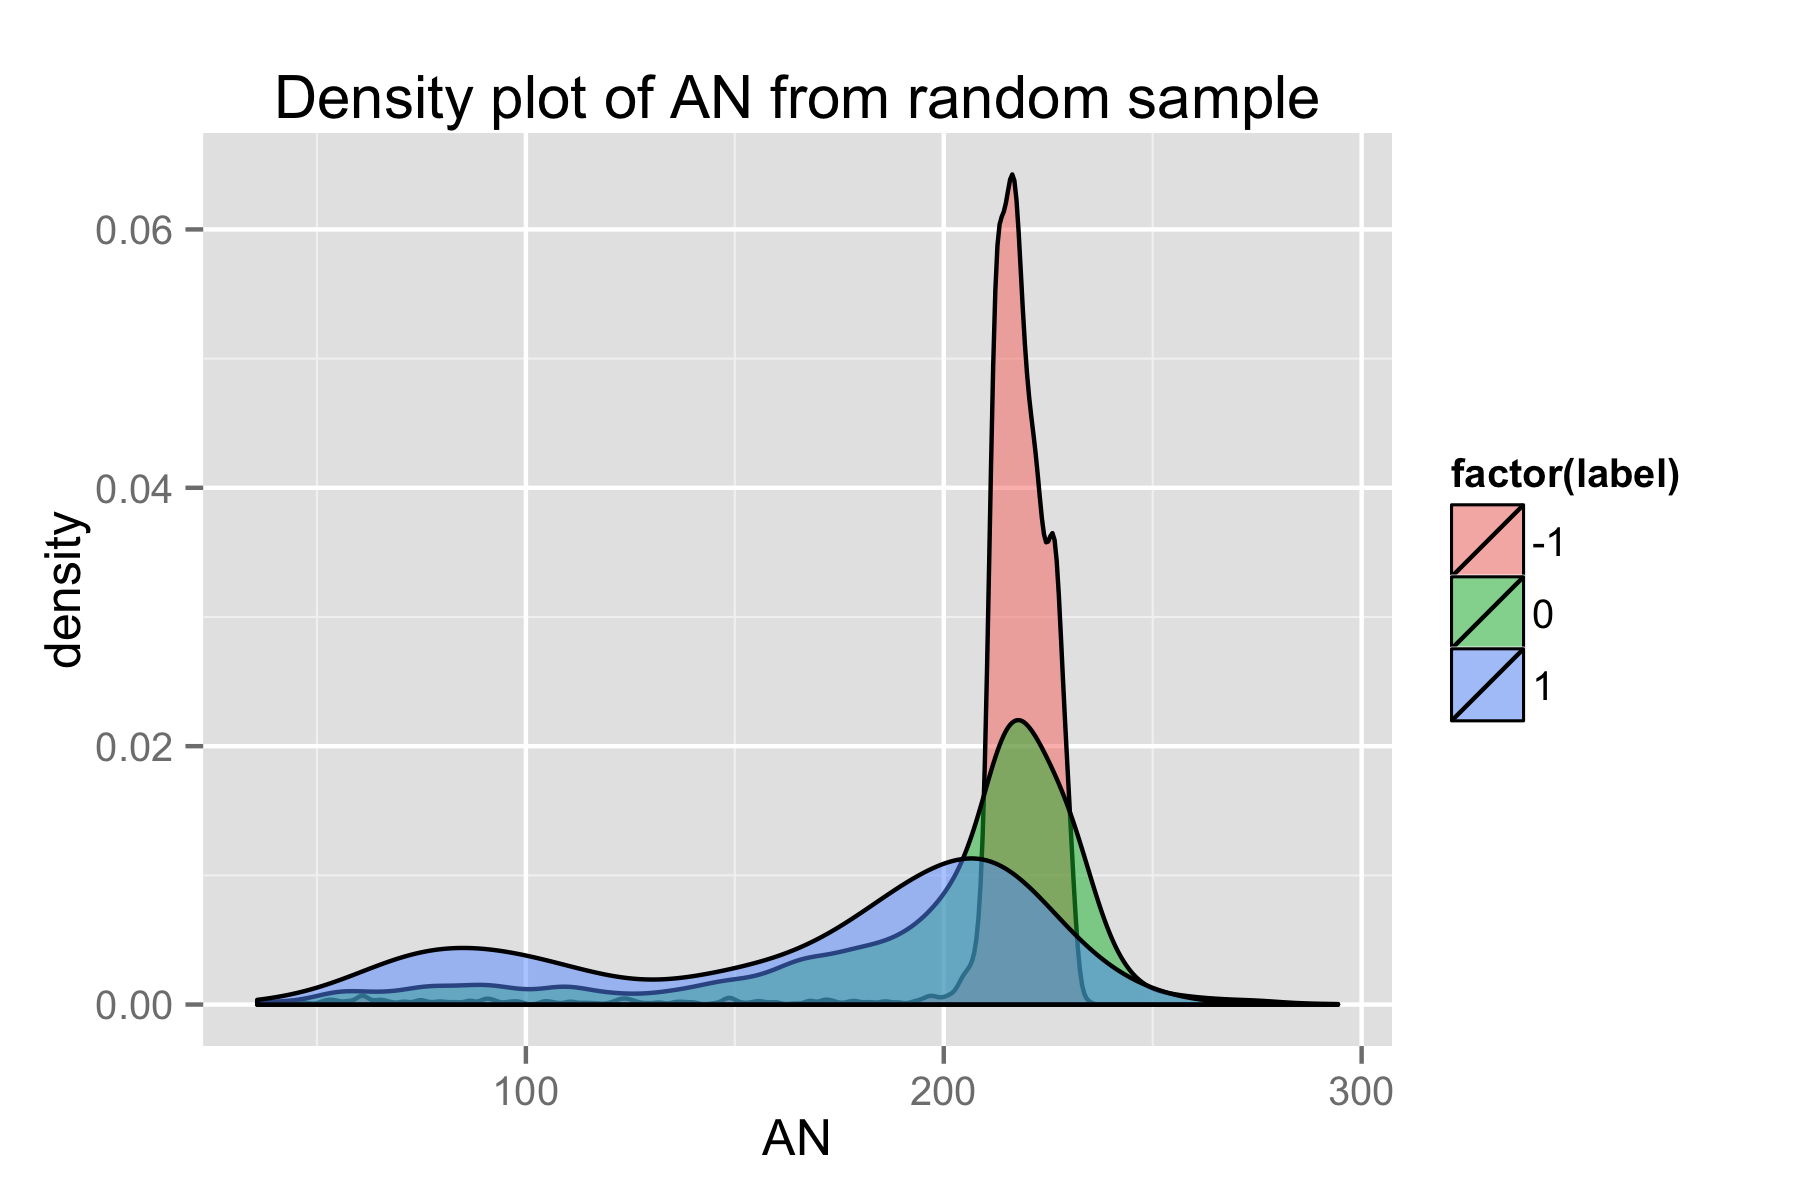
\includegraphics[width=80mm]{../figures/density-AN.png} &
  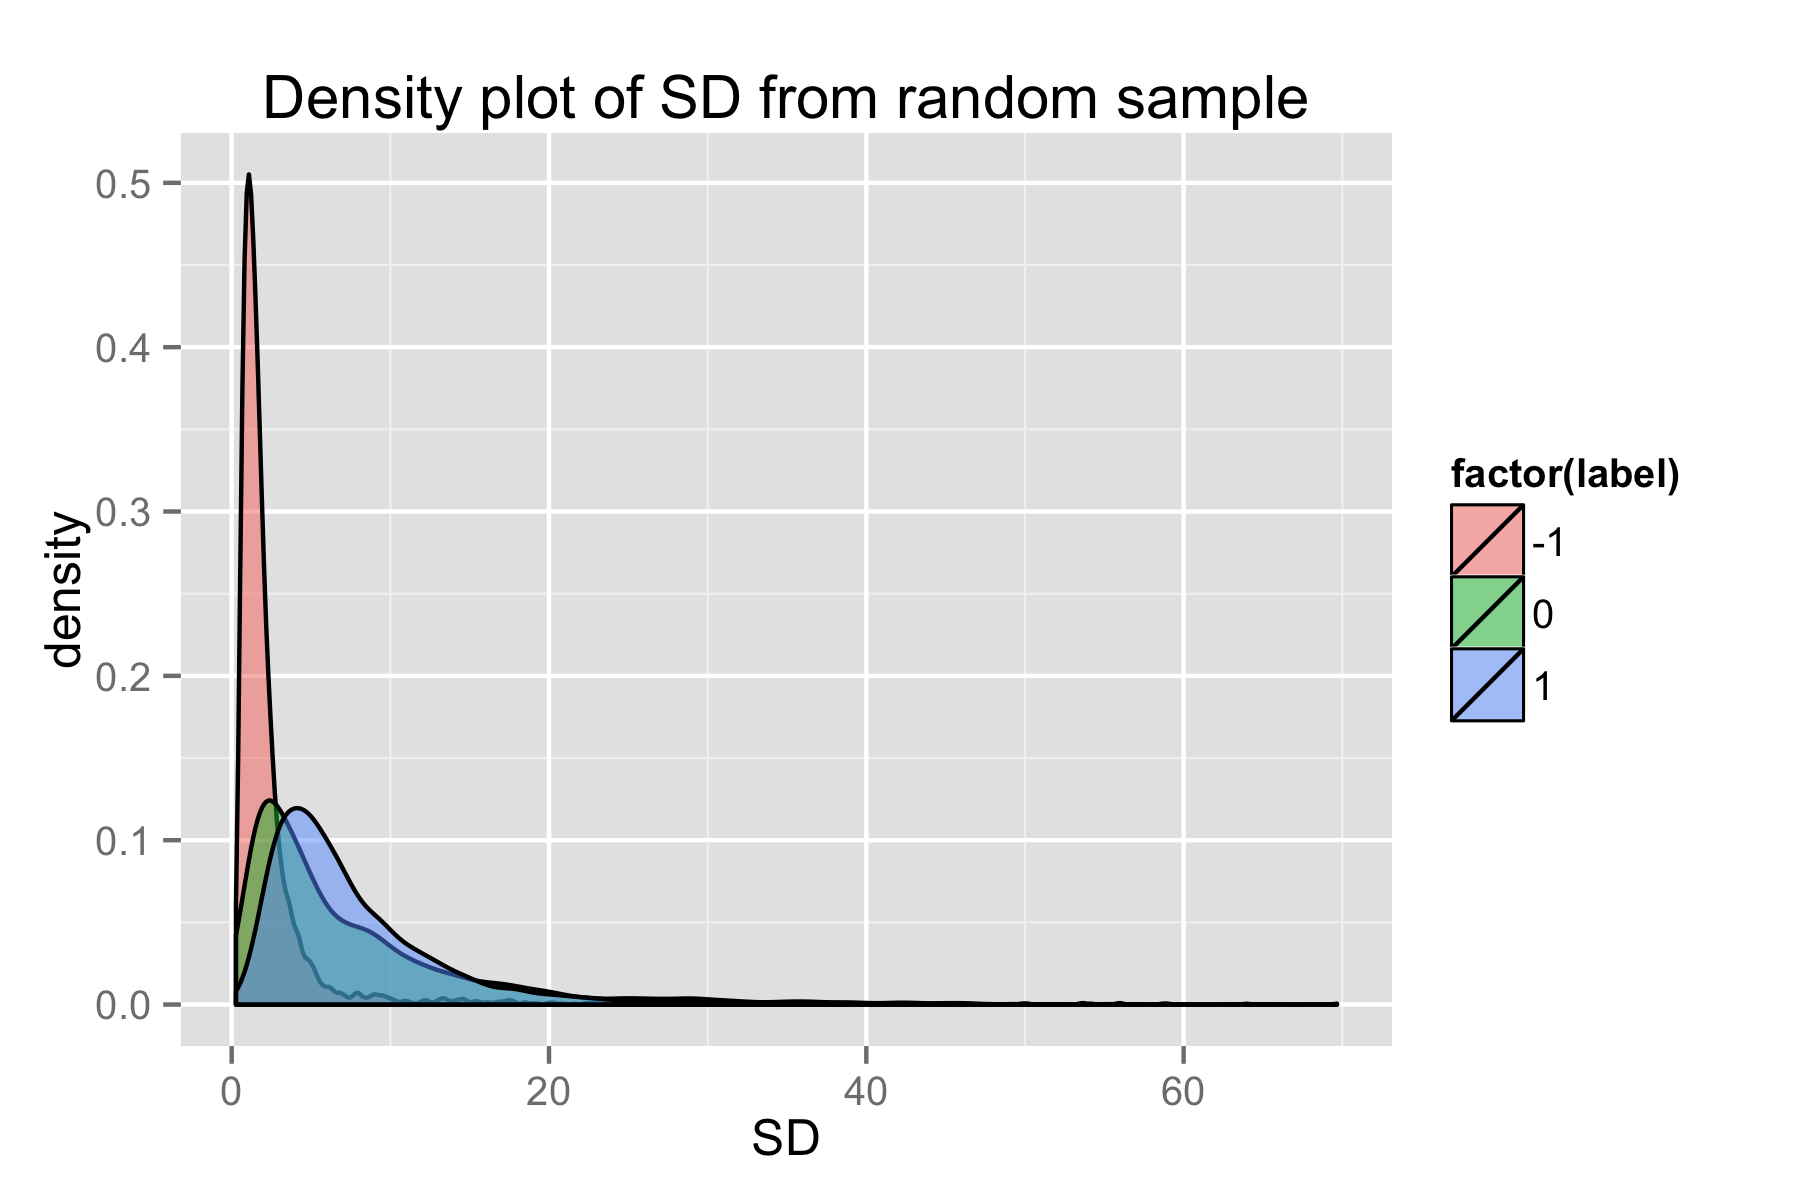
\includegraphics[width=80mm]{../figures/density-SD.png}  \\
  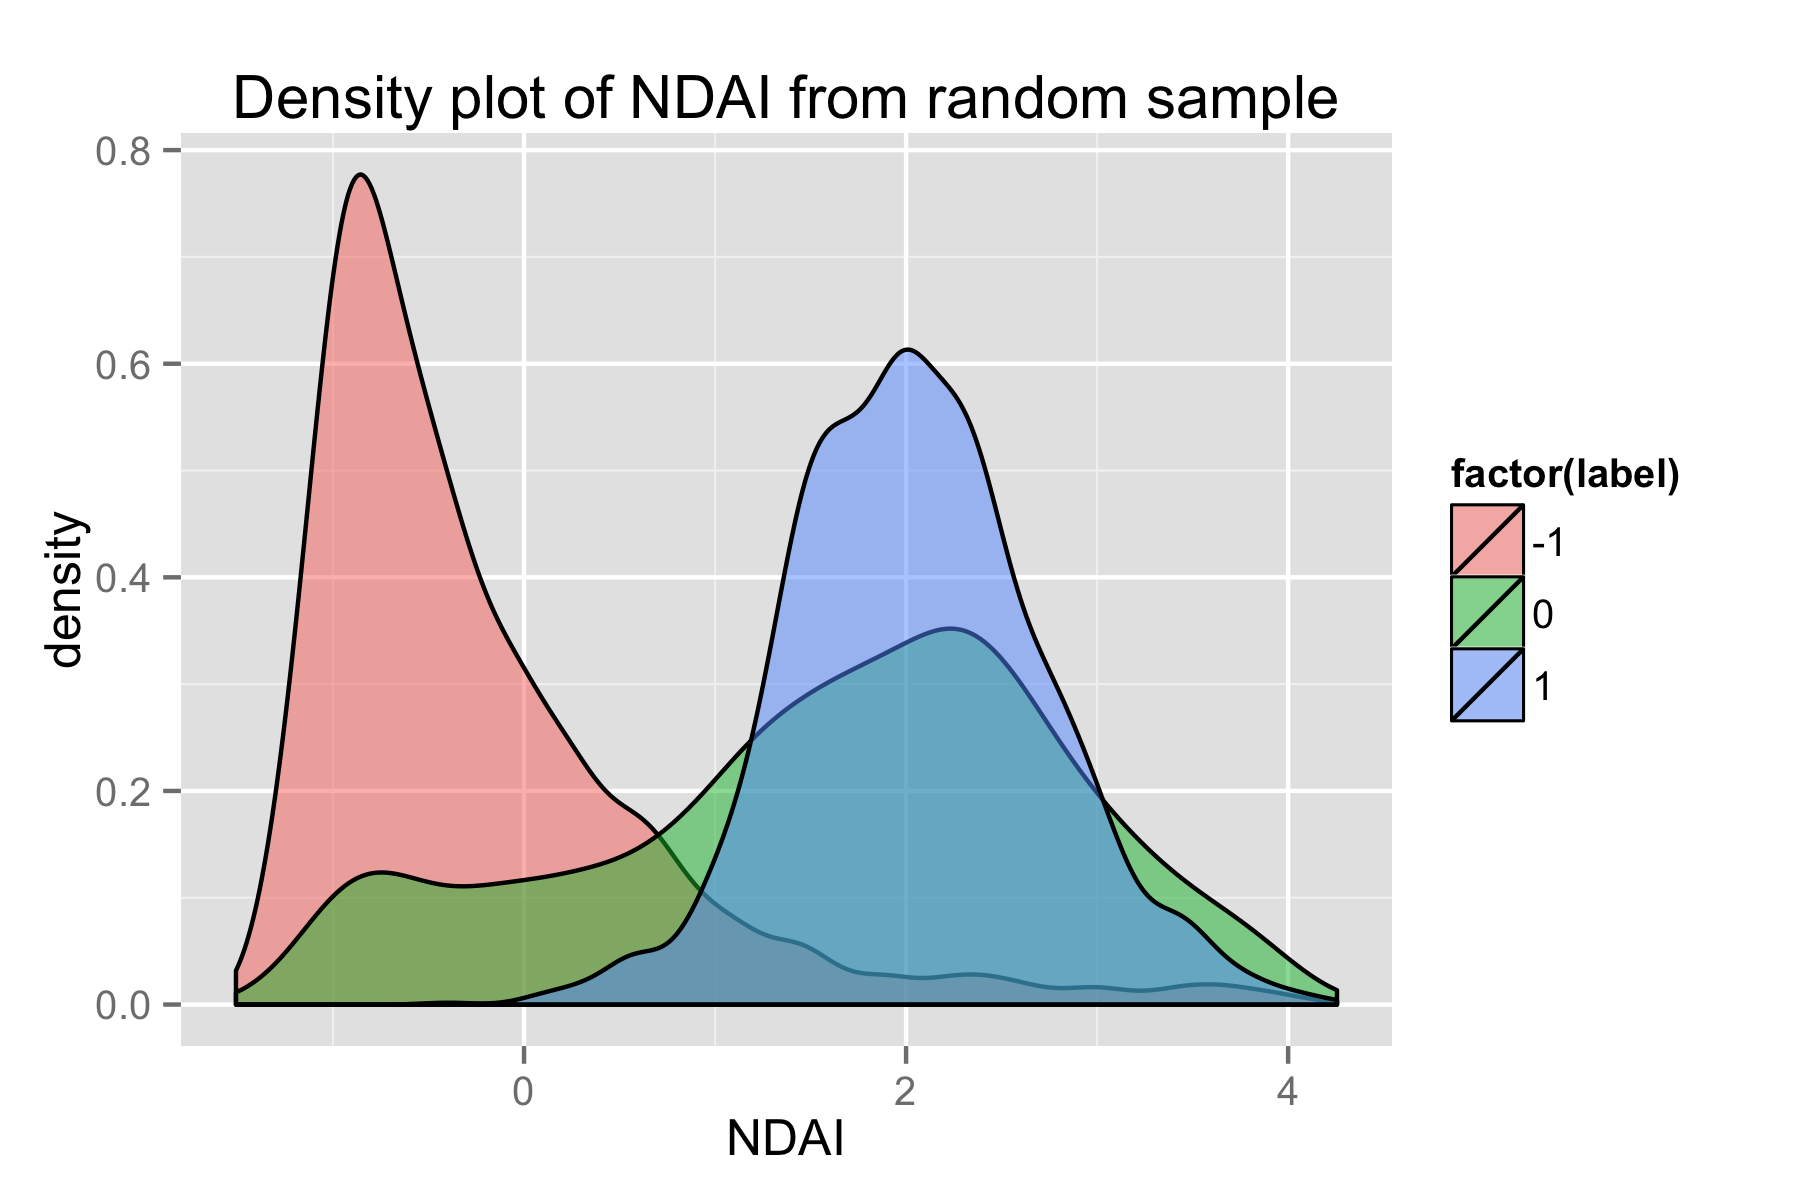
\includegraphics[width=80mm]{../figures/density-NDAI.png} &
  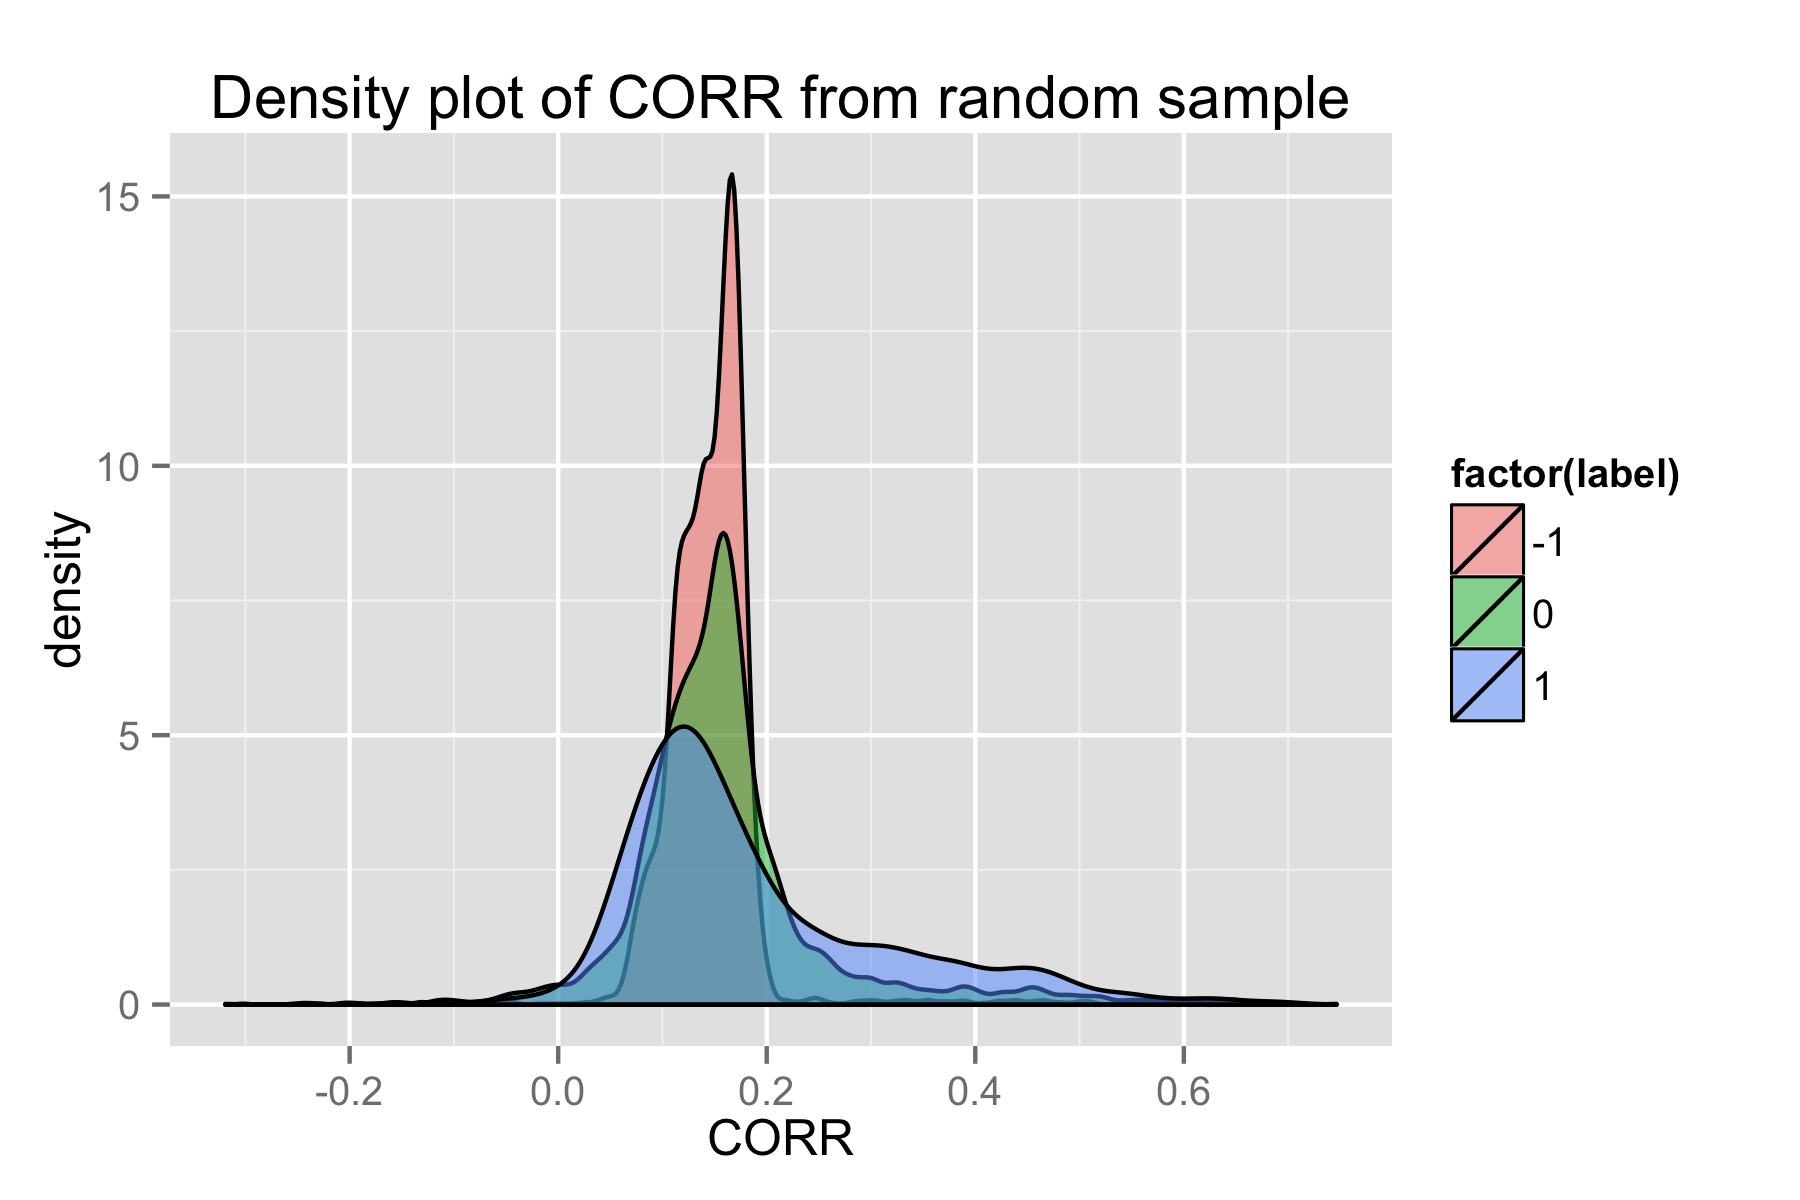
\includegraphics[width=80mm]{../figures/density-CORR.png}  \\
\end{tabular}
\caption{Plots of density, normalized within each category. Ideal features will 
	distinguish the ratio of the likelihood of the ratio of these probabilities, as in 
	a likelihood ratio test. Each of these features possess regions containing 
	notable likelihood ratios for significant amounts of probability mass.}
\end{figure}

NDAI, SD, and CORR have regions with substantial likelihood ratios. Such a 
feature is a good marker for categorization. The bulk of each probability mass 
can be confined to a region of high likelihood by simple threshholding: thus, 
what remains to be seen is whether the probability mass in "questionable" 
regimes can be categorized similarly easily.

\subsection{Scatter Plot Matrix}
The scatter plot matrix for our dataset reveals very strong correlation between
a subset of our elements, yet very little predictive power in this family. This is
the AF, BF, CF, DF, and AN family of data. These features, unfortunately, do
little to shed insight on our categories, and can essentially be boiled down to
one collective variable. There may be a slightly informative subspace within a
linear combination of the variables, but it is far weaker than that of remaining
variables NDAI, SD, and CORR.

\begin{figure}[!h]
  \begin{center}
    \includegraphics[width=\columnwidth]{../figures/splom.png}
  \end{center}
  \caption{Scatter plot matrix shows a highly correlated subspace in the upper 
	right, with several complexly correlated and significantly uncorrelated
	variables on the lower left. By inspection, there could be remaining 
	information in some linear combination of the upper right block (i.e. 
	(NDAI, SD, CORR) x (DF, CF, BF, AF, AN)), but none of the correlated 
	block variables are particularly informative on their own.}
  \label{fig:PT}
\end{figure}

\begin{figure}[!h]
  \begin{center}
    \includegraphics[width=\columnwidth]{../figures/splom_ANhigh.png}
  \end{center}
  \caption{The remaining complexity in this subspace dmonstrates that filtering 
	by AN does not inform our challenging decisions.}
  \label{fig:PT}
\end{figure}

The scatter plot matrix is demonstrated in Fig. ??. It seems like there could be 
important data contributed by the upper-right block to the lower right block. 
However, when we filter on AN, we are left with an "obvious group" -- all low 
AN are easy to categorize, and when we filter on high AN, we are left with the 
original complicated problem of separating NDAI, SD, and CORR, as seen in 
Fig. ??. Thus, we are justified in looking only within the three-feature space of
NDAI, SD, and CORR. This has the additional benefit of making the 
categorization model simpler and more interpretable.

\subsection{Spatial structure}
While we have been currently focusing on pixel-by-pixel categorization, we are
fortunately given additional informative information by virtue of the fact that our
data is taken from spatially correlated variables. Including this spatial data is
crucial: the simple observation that in the expert labels, no cloud label touches
a snow label should indicate the potential efficacy of the inclusion of spatial
information. However, this fortunate observation leads to a wealth of complexity
with regards to how to actually include this spatial data.


\begin{figure}[!h]
\begin{tabular}{cc}
  \includegraphics[width=80mm]{../figures/labels1.png} &
  \includegraphics[width=80mm]{../figures/labels2.png}  \\
  (a) image1.txt labels & (b) image2.txt labels
\end{tabular}
\caption{Expert labels for images show strong spatial structure that can be 
	leveraged for better predictions.}
\end{figure}


A potential route could be to regress each pixel on all of its own data, as well as
on all of its neighbor's data. Another route could be to correct each pixel based
on its neighbor's prior distributions. Our methods will be explored further in our
Modeling section.



\section{Modeling}

\subsection{Feature Selection}
In this section, we perform feature selection in a top-down manner, i.e. we begin with a full set of features, and sequentially remove "ineligible" features from both visual justification by plotting the conditional densities of different features and quantitative exanmination of features' seperability under different conditions using classical permutation test. We also use Akiake Information Criterion (AIC) to measure the relative quality of features, which takes into account both the goodness of fit of the model and the complexity.\\

In order to support classification, features' distributions should have a good separation between distinctive classes. The dissimilarity of distributions can be measured by Jensen-Shannon divergence (JSD), which can be derived from KL divergence and is symmetric distance metric. JSD is given by the following formula:
\begin{equation}
JSD(P||Q) = \frac{1}{2} [KL(P||Q) + KL(P||Q)]
\end{equation}
where $KL(P||Q)$ is the KL divergence, defined as 
\begin{equation}
KL(P||Q) = \sum_i{ln(\frac{P}{Q})P}
\end{equation}
We verify the seperability of a certain feature using permutation test. The idea is to randomly permuate labels of pixels and each time obtain a JSD. The null hypothesis is that the observed JSD for a given feature is independent of the cloud/clear labelings, namely
\begin{equation}
H_0^{Feature}:JSD_{Observed}^{Feature}=JSD_{Permutated}^{Feature}
\end{equation}
The result for permutation test is illustrated in Fig.??, where the histogram is obtained by shuffling the labels for 100 times and the red vertical lines denote the JSD with correct labels. We can see that for features except \textit{AF} and \textit{AN}, the true JSD significantly deviates from the JSD distribution in permutation test. In conclusion, \textit{AF} and \textit{AN} cannot achieve very high seperability and should be pushed out of our feature candidate pool.

\begin{figure}[!h]
  \begin{center}
    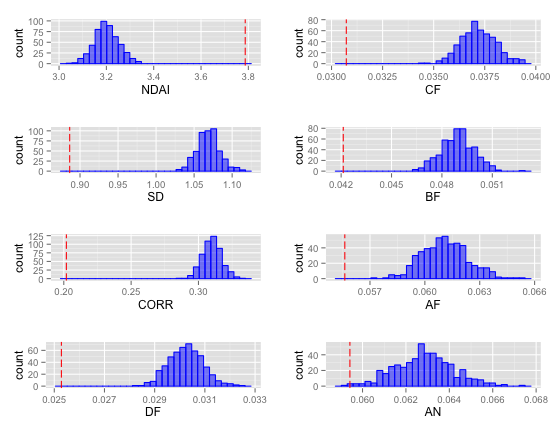
\includegraphics[width=\columnwidth]{figures/PermutationTest.png}
  \end{center}
  \caption{Results for permutation test}
  \label{fig:PT}
\end{figure}

Secondly, we perform a stepwise AIC algorithm on sampled data set (all three images included) to examine the goodness of features. Stepwise AIC is a algorithm to keep tracking the information loss when removing each feature and select the model with the minimum AIC value. The AIC results are shown in Table ??. We can see that removing \textit{AF, BF, CF, AN} results in the least increase of AIC, which indicates that these four features are not very informative and thereby we will remove them from our feature pool.
\begin{table}[!h]
\centering
\begin{tabular}{*{4}{c}}
Features & Df & Deviance & AIC\\
       \hline
<none>   &    & 110896   & 110914\\
- AF     & 1  & 111068   & 111084\\
- BF     & 1  & 111071   & 111087\\
- CF     & 1  & 111103   & 111119\\
- AN     & 1  & 111826   & 111842\\
- CORR   & 1  & 112499   & 112515\\
- DF     & 1  & 112672   & 112688\\
- SD     & 1  & 114236   & 114252\\
- NDAI   & 1  & 168818   & 168834\\

\end{tabular}
\caption{Results for AIC}
\end{table}

From the successive exclusion of features in proceeding steps, we now have four features at hand, namely \textit{NDAI, SD, CORR, DF}. We plot the conditional distribution of these four features (Fig. ??) and it is shown that they all achieve good seperability.

\begin{figure}[!h]
  \begin{center}
    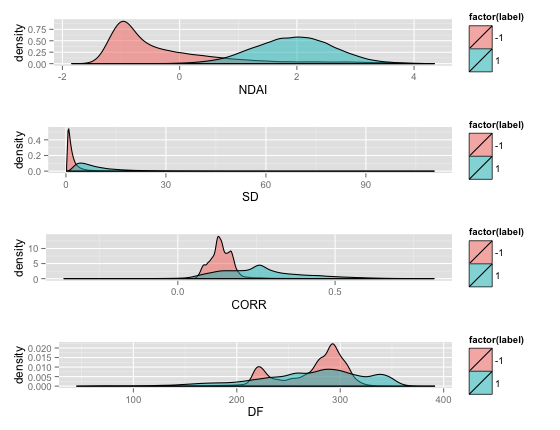
\includegraphics[width=\columnwidth]{figures/ConditionalDistribution.png}
  \end{center}
  \caption{Distributions for NDAI, SD, CORR, DF}
  \label{fig:CD}
\end{figure}

In order to further justify our choice visually, we try to consider combinations of features but reduce their dimentionality to 2D for visualization purpose. Here we repeatly apply PCA to a random sample data set with different combinations of features. In the first trial, we use all features, in the second one only \textit{NDAI, SD, CORR, DF} are incorporated and in the last case the other features are used. From the resulted Fig. ??, where points with different labels are marked differently, we can tell that the second case is the best for classification, since points from two groups are more seperated that in the other two cases. This is a good justification for our choice of features in the feature selection step. In order to make a comparision with result in Bin's paper,  we will proceed our exploration on diverse classification models with four features: \textit{NDAI, SD, CORR}.

\begin{figure}[!h]
  \begin{center}
    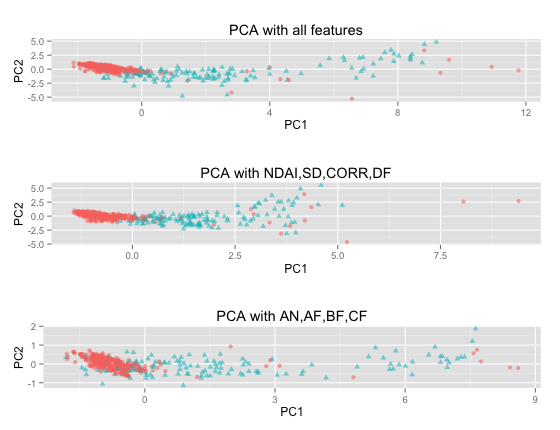
\includegraphics[width=\columnwidth]{figures/PCA_selection.png}
  \end{center}
  \caption{PCA for different combinations of features}
  \label{fig:PCA}
\end{figure}


\subsection{Diverse Classification Models}
\subsubsection{Iterative Conditional Random Field Cloud Segmentation}
We start from the ELCM-QDA model presented in Bin's paper. ELCM-QDA algorithm basically exploits the seperability property of the feature space by thresholding feature values. However, clear and cloudy pixels are not stable in the sense that the feature values might change across time and space. In order to deal with the instability of features, thresholds are chosen by a data-adaptive way, where a mixed-Gaussian model is fitted to the data and the threshold is derived from the dip between two Gaussian distributions. The paper also used Fisher's QDA model to estimate the probability of cloudiness. The result of cloud detection using ELCM-QDA is illstrated in Fig. ??. The agreement with expert labels for three images are $93.39\%$, $93.5\%$, $82.84\%$, respectively. However, if we scrutinize the prediction and the true labels, we can  see that adjacent pixels tend to have the same labels, while ELCM-QDA features a simple thresholding without considering this spatial pattern.\\
\begin{figure}[!h]
  \begin{center}
    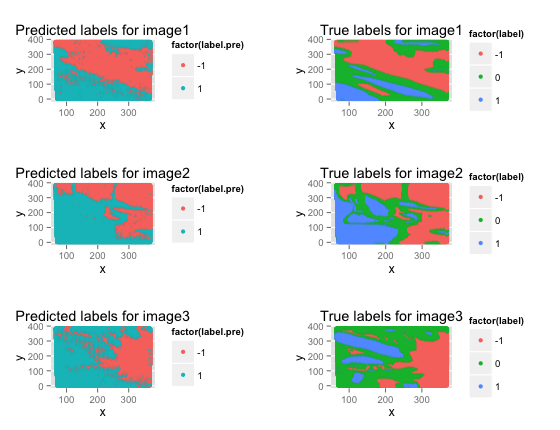
\includegraphics[width=\columnwidth]{figures/ELCMQDA.png}
  \end{center}
  \caption{Classification results of ELCM-QDA}
  \label{fig:ELCM}
\end{figure}
Here we present a Iterative Conditional Random Field Cloud Segmentation (ICRFCS) model which outperforms ELCM-QDA by taking into account spatial homogeneity in cloud images. ICRFCS relies on Bayesian estimation via Markov random field, in which the spatial information in an image is encoded through contextual constraints of neighboring pixels. By imposing such constraints, we expect neighboring pixels to have the same class labels. Let's formalize our algorithm as follows: For each pixel $s$, the region-type that the pixel belongs to is specified by a class label, $w_s$, which is binary in our case, i.e $w_s$ is modeled as a discrete random variable taking values in $\Lambda=\{-1,1\}$. The set of these labels $w={w_s, s\in S}$ is a random field, called the label process. The observed image features are supposed to be a realization $\textsc{F}\{f_s|s\in S\}$ from a another random field,w hcih is a function of the label process $w$. Basically, the image process $\textsc{F}$ represents the manifestation of the underlying label process. Thus, the overall ICRFCS model is composed of the hidden label process $w$ and the observable noisy image process $\textsc{F}$. ICRFCS aims to find an optimal labeling $\hat{w}$ which maximize the posterior probability $P(w|\textsc{F})$, that is the MAP estimate
\begin{equation}
\hat{w}= arg max_{w} P(\textsc{F}|w) P(w)
\end{equation}
According to the derivation in [??], the optimization problem above is equivalent to the following energy minimization problem:
\begin{equation}
\hat{w} = arg min_w U(w, \textsc{F})
\end{equation}
where the energy function $U(w, \textsc{F})$ is given by
\begin{equation}
U(w, \textsc{F}) = \sum_{s\in S} (ln(\sqrt{(2\pi)^n|\Sigma_{w_s}|}) + \frac{1}{2}(f_s-\mu_s)\Sigma_{w_s}^{-1}(f_s-\mu_s)^T) + \beta \sum_{\{s,r\}\in C} \delta(w_s, w_r)
\end{equation}
Minimizing the first term will give us the MLE estimate of labels assuming the features are independent and follow a multi-variate Gaussian distribution. The second term assign greater clique potentials if neighboring pixels have similar classes. $\beta$ is a weighting parameter controlling the importance of local homogeneity. Now, the cloud segmentation probelm is reduced to the minimization of the above function. Since, it is non-convex, combinational optimization techniques are needed to find the global minimum. Due to the computation complexity, we solve this problem in an iterative way. The idea is that we adopt the conventional MLE, while at each step we consider only one pixel and ignore goemetrical considerations and merely choose the optimal by minimizing the energy function assiciated with this pixel. We apply the algorithm until convergence. In our experiment, 5 cycles are enough for the result to be converged.

\begin{figure}[!h]
  \begin{center}
    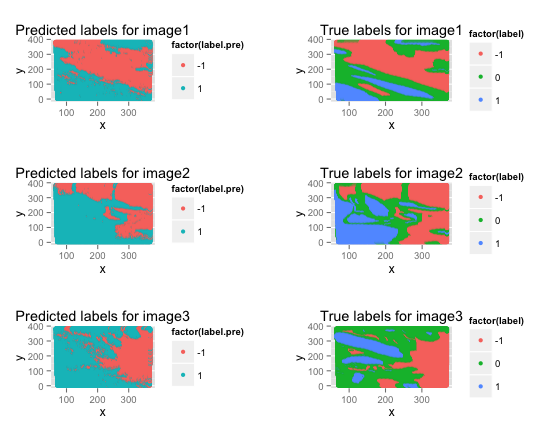
\includegraphics[width=\columnwidth]{figures/CRF.png}
  \end{center}
  \caption{Classification results of ICRFCS}
  \label{fig:ICRFCS}
\end{figure}

The cloud dection result using ICRFCS is shown in Fig. ??. The accuracy of cloud detection for three images are $96.41\%, 95.42\%, 92.24\%$, respectively, which are higher than ELCM-QDA algorithm presented in original paper.

\subsection{Model Assessment}





\end{document}
